\chapter{Introduction}
\label{chap:Intro}

\section{Motivation}
\label{sec:motivation}
Test-Driven Development(TDD) \cite{Beck:03,Astels:03}, a newly emerged
evolutionary software development method, has been accepted by more and
more software developers and intensive research focus has been paid on it
by empirical software engineering researchers. It is said that TDD helps to
have better requirement understanding, reduce debugging effort, improve
productivity, yield high quality code and promote simple
design\cite{Beck:03,George:03,Maximilien:03,Kaufmann:03}. Website
\url{testdriven.com} and user group \cite{TddYahooGroup} are dedicated to
test-driven development community, many tutorial
workshops\cite{OsheroveWorkshop:04,ClarkwareWorkshop:04,AdaptionTddWorkshop,IndustrialLogicTddWorkshop}
and
weblogs\cite{TestDrivenDotComWeblogs,GaryPollice:03,MemoRandaBlog,EichertBlog,MasonBlog}
provide hands-on practice of test-driven development. Modern IDEs Eclipse,
Microsoft visual studio team system, and IDEA already have built-in support
for test-driven development.

Controversially, many benefits of TDD are not backed up by empirical
research \cite{Muller:02,Muller:03,Geras:04}. It is a very interesting
phenomenon that empirical evaluations on tdd are so divided on the fact
that test-driven development is such a plain simple best practice.
Moreover, Kent Beck, the pioneer of TDD, already articulated process of TDD
very well and demonstrated it with Money example in book ``Test-Driven
Development by Example''\cite{Beck:03}.  The persuasive and sound
explanations would be that developers in empirical study did not do
test-driven development, or they did not do it consistently as researchers
expected due to lack of discipline. This is not a hard science problem but
a plain fact because test-driven development radically changes development
``upside down''\cite{Pipka:03} by moving unit testing ahead of
implementation, which is very counter-intuitive to software developers. A
developer tries TDD on a simple problem, he/she thinks TDD is good, and
then he/she forgets it in the future software development and returns to
the old way to develop software.  This story repeats many times already in
the practice of TDD among software developers.

Disciplined test-driven development process is desired in order to conduct
substantial and conclusive empirical research on it. A common problem of
the finished empirical studies on TDD is that there is no better way than
verbal confirmation and participation observation to ensure the necessary
discipline of test-driven development. It will be very interesting and
valuable to have a tool that helps empirical researcher inspect how well
developers do test-driven development automatically and unbiasedly. In the
course of my doctorial research I conjectured, designed and implemented
Zorro software system that can recognize and evaluate test-driven
development automatically.

\begin{comment}
Historically software process research has focused on high-level, long 
duration phases in software development. Recently increasing attention
has been paid to low-level, short duration activities as well. While a
high-level activity such as ``requirement analysis'' might take weeks
to months to complete, a low-level activity such as ``refactor class
Foo to have interface IFoo'' might only take several seconds with modern
IDE. 

Software organizations and developers are continuously confront the needs
to improve their software processes: the software product should meet
customers' requirements better; it should have less bugs; development
process needs to be more stable and predictable; productivity should be
improved to kick the software out of door as early as possible and so on.
Unlike other disciplines such as civil engineering and mechanic
engineering, software engineering is still too young to have mature
software process and quality control process. Software is very cognitive
complicated and software development is a very creative process, thus,
each software is unique and there are no two projects that are exactly the
same. It's challenging to improve software development process.

To a software development organization there are two ways to improve its
development process: one is to identify problems in current process and
solve the problems internally; another one is to adopt successful practices
from others. Internal software process improvement program is often through
process quality control and improvement program. It is heavily emphasized
by SEI's capability maturity model (CMM) and standard ISO9001. Personal
Software Process (PSP) and Team Software Process (TSP) are two processes
proposed by SEI to achieve internal process improvement continuously.
Adopting best practices from others is another way to improve software
process by borrowing others' successful experiences. Usually it comes with
the introduction of new technologies in current development process. For
example, another development tool can be used because it has elegant
features and powerful capabilities; continuous integration can be adopted
to maintain a working version and detect problems early before they sneak
into the final product; software review can be adopted to improve software
quality by peer inspection. Of the two improvement programs, internal
process improvement is gradual and steady, while adopting external best
practice may bring dramatic changes to the development process.

Best practices are from prior successful experiences and they provide a set
of guidelines and recommendations to improve software development. Although
they are proved to be successful elsewhere, they may or may not be
appropriate in a new organization. Managers in the new organizations are
either persuaded by consultants or inspired by other projects' successful
experiences to adopt a new best practice. Introducing best practice is more
or less a trial-and-error approach, and usually the execution discipline is
enforced by management and developers' self-discipline. To software
developers, adopting new best practice is a passive process, and they may
have different opinions as managers do. Everett Rogers modeled new
technology adoption process as adoption curve \cite{Potter:02}, in which
there are five kinds of adopters when a new technology is introduced:
innovators, early adopters, early majority, late majority and laggards.
When a new technology is introduced there is always the learning process
too. Developers may have slow start at the beginning before they understand
the best practice well. Adding these factors together, there will have a
lot uncertainness when a new best practice is exercised such that it is not
possible to tell whether a best practice is appropriate or not in the new
organizations without thorough evaluation. It is fairly reasonable to
conclude that the evaluation process will be more error-prone if the
practice itself is hard to be understood or it has high discipline
requirements.

One may come up with the possible solution to add more management resources
to ensure that the best practices are understood and executed well by
developers, or the development process can be monitored and recorded for
review by process experts.  Although these solutions are viable effective
in manufacture industry, it could be very different to software
organizations. One apparent reason is that software is unique and cannot be
massive produced such that it is very costly to invest management and
monitoring resources on software projects as manufacture industries do.
This puts software organizations in a very awkward situation. On one hand,
it is not easy to employ best practices well to improve software
development process, on another hand, software organizations confront the
needs to improve development process continuously to meet the
ever-increasing demands and dependences on software in our society.

To lower the management overhead of software development, specifically best
practice implementation, we propose to manage and control best practice
execution automatically with micro-process analysis technique in our
research. Micro-process is an innovative approach to keep track of
individual software developer's development process. A framework, software
development stream analysis (SDSA), is used to study micro-processes in
software development.  On the contrary to traditional managerial topdown
approach to enforce process disciplines, SDSA framework takes the bottom-up
step instead. It instruments development process, constructs development
stream out of process data, tokenizes software development stream into
episodes or micro-processes and evaluates development process with
micro-processes. In our research we employ this framework on Test-Driven
Development, a very popular best practice that was formalized and
evangelized by Kent Beck, pioneer of Extreme Programming (XP). Test-Driven
Development is very well accepted by software developers' community but the
researches of Test-Driven Development do not always agree with each other.
Because Test-Driven Development emphesizes on how developers do their work,
it is perfect to apply our framework on TDD to study its micro-processes.
We introduce two terms with our work.
\begin{description}
\item \textit{Software Development Stream} is a series of software
  development activities in order that are conducted by software developers
  over a period.
\item \textit{Micro-Process} is a small set of development activities to
  accomplish one certain programming task. In my proposal I will use both
  episode and micro-process interchangeably.
\end{description}
\end{comment}

\section{Test-Driven Development}
\subsection{Introduction}
\begin{quote}
\textit{Test-driven development (TDD) is emerging as one of the most successful
developer productivity enhancing techniques to be recently discovered. The
three-step: write test, write code, refactor - is a dance many of us are
enjoying. \\
  - Eric Vautier, David Vydra from testdriven.com}
\end{quote}

Test-driven development(TDD), also known as Test-first design(TFD), is a
new way to develop software in which development is driven by automated
unit tests. As its name suggests, TDD radically changes software
development from top-down, design documentation oriented approach to
bottom-up, requirement oriented approach. It has two fundamental
principles\cite{Beck:03}: {\it
\begin{itemize}
\item Write new code only if an automated test has failed.
\item Eliminate duplication
\end{itemize}
} Test-driven development is an incremental and iterative development (IID)
method\cite{Larman:03}. Each iteration lasts several minutes and it is
rarely longer than 10 minutes. In the beginning of an iteration, developer
writes the automated unit test based on requirement. This newly created
unit test may not be able to compile or its execution will fail because it
tests a feature that is not implemented yet. Failed unit test drives
implementation of production code to make it pass. With TDD, a feature is
always accompanied by unit test to guard implementation correctness. The
hidden philosophy behind TDD principles is that developer only writes
enough code to make test pass. If new code adds redundancy developer should
refactor it to remove duplication and keep all tests pass.
Wake\cite{StopLight} uses metaphor stop-light to abstract pattern of TDD
style software development since the unit testing framework xUnit uses red
bar to indicate test failure or error and green bar to indicate test
success and the iterative development manner of TDD works similar as
traffic light.

\subsection{Related work}
``Clean code that works'' is Ron Jeffries's pithy phrase to the goal of
Test-Driven Development\cite{Beck:03}. Since code is driven by automated
tests, system developed in this manner will have 100\% coverage and
developers will have incredible courage to refactor it fearlessly. This
reward is so great that ``most people learn TDD find that their programming
practice changed for good''\cite{Beck:03}. This shift is coined as ``test
infected'' by Erich Gamma. The test in TDD is unit test, a.k.a component
test. Early practice of TDD helped to create xUnit framework, the de facto
standard of unit testing. It was originally designed for SmallTalk and is
already expanded to 35 languages support according to the list on
Wikipedia\cite{xUnit}.

Many TDD advocators appraise TDD because they think TDD helps them improve
productivity and code quality; however, the research conclusions on TDD are
very divided. George and Williams's study got positive results on TDD. They
conducted a structured TDD experiment and compared TDD group who developed
in test-driven development and controlled group who developed in
waterfall-like process \cite{George:03}. Their study found that TDD group
yielded superior external code quality compared to controlled group, but
TDD group took 16\% more time on the development. It is quite interesting
that most TDD developers thought that TDD is effective and improves their
productivity (80\% and 78\% respectively) in the follow-up survey.  Another
study conducted by Maximilien and Williams also reported code quality
increase. Developers reimplemented a legacy software system with TDD in this
study. They found that the new system reduced defect density by 50\% in
functional verification test(FVT) compared to the legacy system that was
developed in ad-hoc manner\cite{Maximilien:03}. There was somewhat
productivity decrease in the experiment but developers inclined to continue
using TDD in their future software development. 

The study conducted by Geras et. al. did not see significant increases on
either productivity and code quality.  They designed an experiment to ask
participants work on two projects with Test-First and Test-Last in
different order in two groups \cite{Geras:04}.  Development effort, tests
per KLOC, customer test invocations and unplanned failures after delivery
were compared between two groups and there was only slight difference
between Test-First and Test-Last processes in both groups. Counter result
was reported by M\"uller and Hagner\cite{Muller:02}.  In their study, TDD
group and controlled group worked on a same graphic library and they
verbally confirmed that Test-First subjects got along with Test-First
process. They found that TDD does not accelerate the implementation and the
resulting programs are not more reliable except that it supports better
program understanding.

\subsection{Problem statement}
Researchers realized that TDD is hard to be done consistently by test
subjects and they tried all they can do to guard TDD discipline in their
experiments. Pair-programming, management, script guideline and verbal
confirmation were ever used in the research to help test subjects do TDD in
the reported empirical studies. The problem is that none of these measures
is efficient enough. Navigator in pair-programming can review the code
constantly and insist driver staying on the track of test-driven
development, but navigator is not always available and many people still
cannot do well on pair-programming. Script guideline and verbal
confirmation are not reliable because developers can go other way around
such as adding unit tests after production code or neglecting unit tests
sometimes. Management of test-driven development is viable but it can only
reach a certain level due to the fact that TDD is iterative and is
constructed of many short-duration activities.

\section{Research statement}
On one hand, TDD is getting more popular among software developers and
intensive efforts have been taken to improve practice of TDD by
professionals and researchers\cite{Beck:03,TestDrivenWeb,TddYahooGroup}. On
another hand, TDD changes software development ``upside down''
\cite{Pipka:03} and is very counter-intuitive to software developers'
problem solving mind-set nature. The result is that it is hard for
developers to do TDD style development consistently and researchers have
hard time to conduct conclusive empirical evaluation on TDD, not even to
mention process improvement.

Test-driven development is a low-level software process that consists of
many short duration activities. This nature determines that traditional
software process management technique can not be applied directly.  The
discipline of low-level software process in general and test-driven
development in particular will largely depend on developer's self control.

Measuring and assessing low-level software process become possible with the
emergence of Hackystat\cite{Hackystat}, a framework for collecting various
kinds of software metrics and developer behaviors. My research attempts to
solve the discipline problems exist in empirical research and practice of
test-driven development with the help from Hackystat. Meanwhile, I
generalize this approach to Software Development Stream Analysis (SDSA)
framework to assist empirical research and practice of other low-level
software processes.

\section{Proposed Solution: Zorro Software System}
The system I develop to assess TDD and improve empirical use of TDD is
called Zorro, which is a multi-layer software system including Hackystat,
Software Development Stream Analysis(SDSA), TDD specific rules, and
applications (Figure \ref{fig:ZorroLayer}).
\begin{figure}[htbp] 
  \centering
  \includegraphics{figs/zorro-layer.eps}
  \caption{Zorro architecture layers}\label{fig:ZorroLayer}
\end{figure} 
Layer 1 is Hackystat that collects product metric and developer behavior
data to be used by upper layers. It also deals with data sending, storage
and encapsulation as data collector. Layer 2 is SDSA framework, which
builds software development stream out of event data and tokenizes
development stream into small episodes, the smallest unit in iterative
software development process in which there is a clear goal and are a
series of development activities. SDSA incorporates
JESS\cite{Friedman-Hill:03} rule-based system to recognize episodes derived
from development stream. Specific rules of TDD are supplied in layer 3 to
recognize and classify episodes of test-driven development tokenized by
test-pass tokenizer. And the fouth layer is application layer which
includes TDD development stream, TDD episode demography, and percentage
telemetry of TDD to assist discipline study and evaluation of test-driven
development.

\subsection{Hackystat}
Hackystat\cite{Hackystat} is an open-source framework developed in
Collaborative Software Development Lab(CSDL) at University of Hawaii for
automated collection and analysis of software product and process metrics
and empirical software engineering experimentation. Hackystat sensors are
small programs plugged into the development environment to collect software
product and process metrics unobtrusively. Hackystat also supplies seamless
data sending, saving and retrieving. A set of analyses on product and
process metrics of software are defined to support evaluations on various
aspects of software engineering. Zorro analysis on test-driven development
compliance extends Hackystat process metric analysis into low-level
software process domain.

\subsection{Software development stream analysis framework}
Software development stream analysis (SDSA) is a generic framework to
analyze low-level software process that are acted by development
activities such as file editing, compilation, testing and debugging. SDSA
retrieves low-level development activities collected by Hackystat sensors,
constructs development stream by serializing these activities, defines a
set of tokenizers to organize related activities into episodes and
implements an interface to recognize episodes with rule-based system
support.

SDSA is a component-based system and is highly configurable. End users of
SDSA can selectively add sub stream, the unified development stream with
one single type of activities, into the main development stream. It defines
interface to plug in different episode tokenizing mechanisms and allows end
users define episode recognition rules by themselves.

\subsection{Recognition rules of Test-Driven Development}
Test-driven development is an iterative and incremental method, each
iteration consists of three portions red/green/refactor. Zorro instantiates
SDSA framework and selects test-pass tokenizer to have software development
episodes that end with successful unit test execution(s). A TDD iteration
will be separated into two portions red/green and refactoring, both of
which end with successful unit tests invocation. An episode is refactoring
if there is no new test and it is red/green if there is new test added. A
red/green episode is test-driven if and only if development is driven by
unit test.  So it can be further divided as test-driven in which unit test
is created to drive product code implementation, and test-last in which
unit test is created after the production code implementation. Complete
classification tree of test-pass episodes is depicted in Figure
\ref{fig:EpisodeTree}.
\begin{figure}[htbp] 
  \centering
  \includegraphics{figs/EpisodeClassficationTree.eps}
  \caption{Zorro test-pass episode classification tree}\label{fig:EpisodeTree}
\end{figure} 

\subsection{Zorro applications}
Zorro has a very simple interface that displays software development stream
of TDD in episodes \ref{fig:zorro-gui}. Demography of TDD episodes is
another application that illustrate distrubution of Zorro episode
categories in blocks, pie chart and box-whisker chart. 

Software telemetry\cite{csdl2-04-11} is an approach to manage software
development and it provides project members and manager insights useful for
local, in-process decision-making. Zorro implements telemetry reduction
function to assist parallel correlation between test-driven development and
other attributes such as code coverage, active time, or other software
metrics. By combining low-level software process detection and software
telemetry, we will have a very powerful mechanism to assit evidence-based
software engineering \cite{Kitchenham:04}.

\subsection{Contribution of Zorro}
Test-Driven Development has been claimed to naturally generate 100\%
coverage, improve refactoring, provide useful executable documentation,
produce higher code quality and reduce defect
rates\cite{Beck:03,George:03,Maximilien:03}. The multi-layer structure I
propose can automate collection of developer behavior data and test-driven
development recognition. If it recognizes TDD correctly, then we would have
a powerful mechanism for exploring how test-driven development is used in
practice and its effect on software quality and productivity. The
non-intrusive nature of data collection provided by Hackystat will make it
very easy to deploy Zorro in both classroom and industrial settings to
study TDD compliance (management), potential discovery of alternative
processes and investigation of impacts of TDD.

\section{Zorro validation studies}
Before Zorro can be used in the practice and empirical research of TDD, it
must be validated to sustain that (1) it can collect the software metrics
and developer behavior data necessary to determine TDD, and (2) it can
recognize TDD correctly with the collected data. A pilot validation study
on Zorro was conducted in University of Hawaii in spring 2006. An extended
validation study in classroom setting and another validation study with
experienced TDD developers are scheduled in fall 2006.

\subsection{Pilot validation study}
A pilot validation study of Zorro was conducted in University of Hawaii in
spring 2006. We recruited 7 experienced java developers and asked them
implement a stack data structure in Eclipse IDE with test-driven
development method following the provided TDD tutorial and implementation
guideline. Process of the study was instrumented by Hackystat Eclipse
sensor for collecting development event data.

We realized that it is necessary to have another independent data source to
compare data collected and analyzed by Zorro. An Eclipse plug-in, Eclipse
Screen Recorder(ESR), was designed and implemented to record changes of
Eclipse window caused by development activities into a QuickTime
movie\cite{csdl2-06-02}. Because ESR can sincerely record development
activities, we will have an independent high fidelity data source to
validate developer behavior data collected by Zorro. Also we can use the
recorded video to validate Zorro episode recognition results. Figure
\ref{fig:PilotSummary} presents this pilot validation results in a table.
\begin{figure}[htbp] 
  \centering
  \includegraphics{figs/Pilot-Summary.eps}
  \caption{Summary of pilot validation study}\label{fig:PilotSummary}
\end{figure}
 
The pilot study demonstrated that Zorro can collect complete enough
developer behavior data to recognize test-driven development and the
recognition accuracy is close to 90\% percent
(figure\ref{fig:PilotSummary}). However, 10\% episodes were wrongly
classified due to incomplete data and insufficient TDD recognition rules.
Causes were identified and improvements were made after the pilot study.

A provoking finding of pilot study is that developers spent quite some time
doing test-last development (on the contrary to test-driven development),
even though they knew it was a study on test-driven development and the
guideline on TDD implementation of stack was available for reference. Our
conjecture is that it could be caused by the simplicity of stack problem or
nature of test-driven development. Further studies on more complicated
problems with experienced TDD developers must be conducted to have more
comprehensive validation on Zorro.

\subsection{Case study in Classroom}
An extended Zorro validation study is going to be conducted in a software
engineering class in fall 2006 to validate Zorro's data collection and
recognition of test-driven development as in the pilot study. Students will
be taught unit testing and test-driven development before they take
participant in this study. The development process will be instrumented by
Hackystat Eclipse sensor to collect developer behavior data for Zorro
assessment and ESR to record students' development process.

\subsubsection{Materials}
Programming language is Java and Eclipse is the only IDE supported in this
study. Students will learn modern software engineering knowledge and
development techniques including JUnit, Eclipse and test-driven
development. They will be participating this case study by practicing TDD
with one the the following three problems and do some test-driven
development on their course projects.
\begin{enumerate}
\item{Roman numeral converter: a program that can convert any integer
    number between 1 and 50 into its Roman numeral.}
\item{Bowling score calculator: a bowling game contains 10 frames, each has
    2 maximum throws to knock down as many pins as possible. Score of a
    bowling game is the sum of each frame and bonus if applicable.}
\item{Stack: a data structure that works in Last-In-First-Out(LIFO)
    principle.}
\end{enumerate}

\subsubsection{Data collection}
Hackystat Eclipse sensor will be used through the entire study to have
collect developer behavior data. Practice of TDD and the mandatory software
development process will also be instrumented by ESR to collect development
process video.

\subsubsection{Experiment procedure}
The classroom case study of Zorro consists of training, TDD practice TDD
enactment and course project development.

\paragraph{Training}
Considering that students are new to test-driven development and they are
lack of unit testing skills, we allow a skill building process at the
beginning of the semester. Apart from fundamental knowledge of software
engineering, students will also learn modern software development tools
such as Eclipse, subversion, ANT, JUnit, and software development
techniques such as coding standard, MVC pattern, test-driven development.

\paragraph{Practice of test-driven development}
I prepared three problems roman numeral converter, bowling score calculator
and stack with step-wise tutorial of test-driven development implementation
for students. Every student takes one of them to practice and their
development process will be instrumented by Hackystat Eclipse sensor and
ESR.

\paragraph{Enactment of test-driven development}
Students will be assigned a course project to implement and they must do
test-driven development in the first week with at least 3 hours' active
time. Again, this process is instrumented by Hackystat Eclipse sensor and
ESR.

\paragraph{Course project development}
After the first week's mandatory test-driven development, it is up to
students to choose whatever process works best for them in their course
project development. Of course students can still do test-driven
development on their own choices. Only Hackystat Eclipse sensor will be
used to instrument the course project development. 

\subsection{Case study within TDD community}
Eventually Zorro is supposed to help discipline study and management of
test-driven development in practice. Case study in academic setting suffers
external validity problem, we must run multiple studies\cite{Yin:03} to
generalize the validation results of classroom case study of Zorro. With
the resource available for my Ph.D research, it could be viable to reach
experienced TDD developers of test-driven development community.

\subsubsection{Test subjects}
The best way to reach experienced TDD developers is through TDD community,
website \textit{testdriven.com} and TDD user group \cite{TddYahooGroup}. I
will solicit participation in the study of experienced TDD developers by
evangelizing Zorro software system into the community with the hope that
they can see the benefits of it in their professional software development.

\subsubsection{Data collection}
The unobtrusive data collection manner of Zorro and intuitive process
recording tool ESR\cite{esr} should make the participants painless to
configure the testing environment. Hackystat provides a DocBook chapter of
Zorro case study guideline\cite{Hackystat} to assist developers on
configuring testing environment.

\subsubsection{Experiment procedure}
Participants will do test-driven development on their own with
instrumentation of Hackystat Eclipse sensor and ESR. To encourage
participation, test subjects can choose the problem they want to work on
in test-driven development. Problem candidates are:
\begin{itemize}
\item One problem from problemset of stack, roman numeral converter and
  bowling score calculator.
\item Another interesting problem such as Money example, Sudoku or
  Spreadsheet.
\item A test-driven development session at work.
\end{itemize}

For Zorro validation, we suggest developer working on the chosen problem in
test-driven development for more than half an hour. Developers can send
their ESR movies to me for data analysis. A summary of the analysis result
will be avaulable for them as reference.

\subsubsection{Validation analysis}
Developer behavior data and ESR video are two data sources for analysis. A
Zorro project can be configured to every test subject to run Zorro
analysis. Similar as pilot study we will use the recorded video to validate
the collected behavior data and the recognition results. 

\section{Contribution}
I proposed software development stream analysis (SDSA) framework to study
low-level software process with very fine-grained developer behavior data.
Unlike traditional software process research that treats software process
as either a rigid process defined by formal methods or a stochastic
process, SDSA adopts the mix of bottom-up and top-down method to assess
the compliance of low-level software process with rule-based system
support. It introduces a new and executable way to automate process
comformance evaluation.

The software system out of this research work is Zorro. If the validation
studies agree that Zorro can collect complete enough developer behavior
data and recognize test-driven development correctly, the TDD community and
researchers will have a very powerful full to improve TDD practice and find
ways to improve it. The possible uses of Zorro in test-driven development
process mangement and training will greatly improve the discipline of TDD
in practice and education. Other than compliance assessment of test-driven
development, the rich developer behavior data collected in the development
process can be used for other research such as development pattern
search.

Another contribution of this research will be the Eclipse Screen Recorder
(ESR), the data validation tool. It can be used to conduct developer
behaviors related research such as peer software review process observation.

\section{Roadmap}
This thesis work introduces Zorro software system for recognizing
test-driven development to improve practice and empirical evaluation of it
with software development stream analysis technique. Chapter
\ref{ch:relatedwork} briefly goes over literature work on test-driven
development and automation of software process research. Zorro architecture
and the implementation details are addressed in chapter
\ref{ch:implementation}. Case studies to validate Zorro are described in
chapter \ref{ch:evaluation}.

\begin{comment}
\section{Software Development Stream Analysis Framework}
At the very beginning software development was ad-hoc and software
projects' successes largely depended on the talents and capabilities of
individual programmers. The introduction of software process such as
waterfall model changed the route of software development from chaos into
discipline. In definition, software development stream is a series of
software development activities in chronological order that are conducted
by developers over a period. Since these activities track what programmers
do, we can say that software development stream reflects how developers
execute software process. It is great to have software development stream
but we do not end up with it because one development stream can be very
long and has too many activities. The massive information it contains
and analysis complexity of software development stream inspired us to
develop micro-process, a small portion of the software development stream
to accomplish a programming task. Like microscope to magnify objects,
micro-process provides a very detailed view on software development
process. It introduces a very adequate way to analyze software process as
well as best practice in software development.  Software development stream
analysis framework binds development stream and micro-process together. It
includes activity data collection, development stream construction,
episode recognition and evaluation as well.

\subsection{Software Development Stream Construction}
In the course of software development, developers interact with tools to
produce software artifacts. The data collection system will have to collect
both development activity data and software metrics to keep track of the
software product changes. Process data are either developers' direct
interactions with tools or the program's changes committed by developers.

Our data collection is supported by Hackystat, an in-process unobtrusive
metric collection system. Hackystat has more than 10 sensors to collect
development activities, software metrics, unit test, build, file commits
and so on. Hackystat stores process metric data in a centralized server in
XML format. We reduce raw software metric data into activities directly or
indirectly by checking continuous software metric variations. For
convenience reason each activity type is processed separately to form
development sub steam, which has homogeneous activities only. We merge sub
streams together to create software development stream.  Table
\ref{tab:stackstream} is part of the software development stream whilst I
worked on a stack data structure implementation.
\begin{table}[!h]
\centering
  \begin{tabular}{|llll|}
  \hline
    23:43:57 & TestStack.java & ADD CLASS & package org.sci \\
    23:43:57 & TestStack.java & ADD IMPORT & import junit.framework.TestCase \\
    23:43:57 & TestStack.java & MOVE CLASS & org.sci --\textgreater TestStack.java \\
    23:44:19 & TestStack.java & ADD METHOD & void testEmptyStack() \\
    23:44:38 & TestStack.java & TEST EDIT & 6sec \\
    23:44:39 & TestStack.java & COMPILE & Stack cannot be resolved \\
    23:45:07 & Stack.java     & ADD CLASS & Stack.java \\
    23:45:07 & Stack.java     & BUFFTRANS & FROM TestStack.java \\
    23:45:34 & Stack.java     & ADD METHOD & Stack() \\
    23:45:56 & Stack.java     & PRODUCTION EDIT & 18sec \\
    23:46:02 & TestStack.java & BUFFTRANS FROM & Stack.java \\
  \hline
  \end{tabular}
  \caption{Development Stream Example}\label{tab:stackstream}  
\end{table}
Stack works on the principle of Last-In-Last-Out(LILO). I implemented stack
in Java with best practice Test-Driven Development (TDD). The
implementation starts with test object \textsf{\textbf{TestStack.java}} to
drive the implementation of stack. Test case \textsf{\textbf{void
    testEmptyStack()}} is added right after since it is an easy task to
test and implement. The compilation of the test class failed because object
\textsf{\textbf{Stack}} does not exist yet. The rest of the work is stack
emptiness check. This is a typical TDD-style development scenario that can
be replayed by software development stream.

\subsection{Best Practice Tokenization and Identification}
Development stream has rich information on software process. It's easy to
analyze a small portion of the development stream, but it is not feasible
to look up the real development stream because it may have thousands of
activities. The identification and evaluation of best practices with
development stream must be done automatically. There are some literature
work on automatic software development process discovery and modeling. Cook
et al \cite{Cook:95} implemented a system called Balboa to discover and
validate formal software process with finite state machine.  Chris Jen et
al automate discovery and modeling of open source project development by
studying web activities with email, message board and instant messaging
etc\cite{Jensen:04}.

Software development best practice contains a set of rules and
recommendations to regulate development process. It either defines the
order of development activities or adds new pieces to the development
process. For example, incremental build is the best practice to audit
developers' edit work and build system once there are changes being made;
unit test best practice emphasizes that developers should write their unit
tests to improve the quality of their programs. Because best practices are
repeated in development process, the software development stream should
contain many best practice iterations when it is deployed. Our strategy is
to tokenize development stream into iterations, which can also be called
micro-process or episode.

An episode contains a series of activities following the best practice if
developers comply the rules and recommendations of it. Rule-based system is a
natural choice to identify the execution of best practice. In a rule-based
system knowledge is represented in the form of \textit{if...then...}
rules\cite{Luger:02}. The inference engine in rule-based system can apply
best practice rules on development episode to identify best practice.
Figure \ref{fig:concept} illustrates the concept and infrastructure of this
recognition system.
\begin{figure}[h]
  \centering
  \includegraphics{figs/ConceptStructure.eps}
  \caption{Episode Recognition System}\label{fig:concept}
\end{figure} 
It provides a powerful tool to identify and evaluate the execution of best
practice without human being's intervention.

Software Development Stream Analysis (SDSA) framework unites data collection, 
development stream, episode tokenization and episode identification together 
to study best practice in software development. In my thesis work I apply this 
framework on best practice Test-Driven Development, a practice of Extreme 
Programming (XP).

\subsection{Test-Driven Development Process Measurement}
\subsubsection{TDD Episode Tokenization}
Red/Green bar is the pattern of Test-Driven Development. It implies that an
episode ends with successful unit test execution, the green bars are tokens
of Test-Driven Development. We define {\it Test Pass Tokenizer} to partition
development stream in the context of Test-Driven Development. It ends an
episode when there is a successful unit test execution, figure
\ref{fig:testpass} is one test-pass episode example.
\begin{figure}[h]
  \centering
  \includegraphics[width=0.9\textwidth]{figs/TestPassEpisode.eps}
  \caption{Test Pass Episode}\label{fig:testpass}
\end{figure} 

Technically test-pass tokenizer is enough to detect iterations of
Test-Driven Development. However, in team software development, developers
also deploy their work with the whole system to make sure new code will not
break it before integration. To accommodate team software development we
defined \textit{Commit} and \textit{Command} tokenizers for integration and
deployment activities. On the other side, developers may not do TDD or
occasionally step away from TDD without frequent unit test invocations. We
defined \textit{Buffer Transition} tokenizer to divide this kind of
micro-processes into smaller buffer transition micro-processes for further
analysis.

\begin{itemize}
\item \textit{Commit tokenizer} ends an episode when it encounters a bunch
  of file commit activities. It can be used to inspect what developers do
  before integration.
\item \textit{Command tokenizer} ends an episode when there are some
  consecutive command build activities to deploy system in local
  environment.
\item \textit{Test Pass tokenizer} ends an episode when there are
  successful unit test invocations. We implemented it to find the iterations
  in Test-Driven Development.
\item \textit{Buffer Transition tokenizer} starts an episode when it
  encounters consecutive buffer transition activities. It sums what
  developers did to the working buffer.
\end{itemize}

\subsubsection{TDD Episode Identification and Classification}
Test-pass tokenizer partitions development stream into many iterations that
end up with successful unit test execution. In term of TDD, a test-pass
episode can be either ``test-driven'' or ``refactoring''. The significant
property of refactoring is that there is no new test case in refactoring 
episode. With this character we can classify test-pass episodes of TDD into 
two categories, ``test-driven'' and ``refactoring''.  Moreover, a test-pass 
episode with test creation may or may not be ``test-driven''.  Test-Driven 
Development implies the order of development is to ``test a little, code a 
little and repeat."\cite{Beck:03} such that it will be ``test-last'' if test 
is not created before code implementation. Figures \ref{fig:tdd} and
\ref{fig:refactoring} illustrate different kinds of ``test-driven'' and 
``refactoring'' episodes respectively.

\begin{figure}[h] 
  \centering
  \includegraphics[width=0.8\textwidth]{figs/TDD.eps}
  \caption{Test-Driven Episode Classification}\label{fig:tdd}
\end{figure} 

\pagebreak
\begin{figure}[h] 
  \centering
  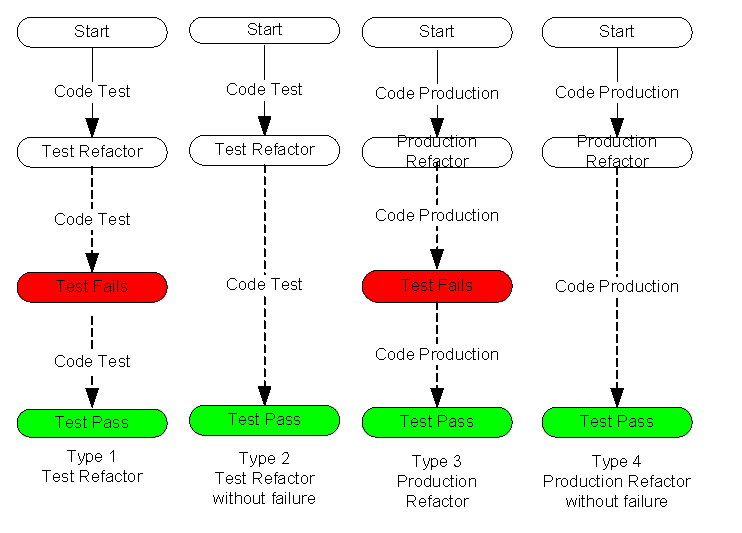
\includegraphics[width=0.8\textwidth]{figs/Refactoring.eps}
  \caption{Refactoring Episode Classification}\label{fig:refactoring}
\end{figure} 

 as in Figure \ref{fig:EpisodeTree}.
\begin{figure}[htbp] 
  \centering
  \includegraphics[width=0.8\textwidth]{figs/EpisodeTree.eps}
  \caption{Episode Tree}\label{fig:EpisodeTree}
\end{figure} 

Some empirical case studies \cite{George:03}, \cite{Maximilien:03}
reported successes on TDD practice. According to these studies TDD group
passed more black box tests than TLD group and they spent less time on
projects than TLD group. Even though most empirical studies drew positive
conclusion on Test-Driven Development there are still some neutral or
negative reports on TDD. Geras etc. \cite{Geras:04} found that there is
little or no difference in developer productivity in TDD and TLD processes.
Another study \cite{Muller:02} concluded that TDD does not accelerate the
implementation and the resulting programs are not more reliable than TLD.

\section{Validation}
Unlike many other cumbersome software processes such as Spiral model, PSP or
RUP Test-Driven Development is very lightweight. It contains two simple
rules only. In practice TDD is hard to follow compared to other processes
because there is no management involved in the development. In situations
that pair programming is not involved developers are fully responsible for
TDD execution by themselves without monitoring. This weakness will bring
many questions to TDD process. Do developers do Test-Driven Development
when they are told to do so? And if they do how well they do TDD in their
development? Do developers always follow two TDD rules?

In my thesis study I will build a system on top of Hackystat to answer
these questions as well as provide a tool to discipline TDD process.  There
are two goals to pursue in my work. One is to study how the development is
being done, especially how the unit testing is conducted in Test-Driven
Development. Another goal is to study properties of TDD. Will developers
spend more time on development and yield high quality code or not? Will the
test coverage be naturally 100\%?

Scott Ambler's UML diagram (Figure \ref{fig:TDDSteps}) depicts TDD development
iterations.

\begin{figure}[htbp] 
  \centering
  \includegraphics{figs/TDDSteps.eps}
  \caption{The Steps of TDD}\label{fig:TDDSteps}
\end{figure} 

\begin{itemize}
\item The first step is to add a test quickly. Basically it just fails the
  code.
\item Next run your test or test suite to make sure the new test does fail.
\item Make changes to the function code to make test pass. As long as it
  can make test pass you even can fake the implementation, for instance,
  return a constant number.
\item Run your tests again. If it still fails you go ahead to update your
  function code. Once all tests pass you can start over with a new test.
\end{itemize}

In the early era of software development there is no software process.
Software systems are developed in a chaotic style and their successes
depended largely on individual's skills and capabilities. Water-fall model
is the first and most popular software development process and it still
exists in many organizations. In water-fall model software development is
divided into stages from requirement analysis to operation and testing is
conducted after project is implemented. Bugs and defects found in testing
will be fed back to the development team or maintenance team. Since bugs
and defects are revealed at the late stage of software development
water-fall model is reluctant to meet customer's requirements and defect
fix. If defects are rooted from design it will be extremely hard to adapt
changes according to water-fall model.

Modern iterative incremental development(IID) was developed to fix this
problem by dividing a large project into many parts.  They are implemented
iteratively. Each iteration can be a mini-waterfall process so that defects
can be fixed and changes can be made very quickly.  Spiral model is the
first process definition to formulate iterative incremental development
practice. Other variations like prototyping, RAD, CleanRoom, Scrum, RUP,
FDD, Extreme Programming are used in many projects successfully.  Latest
development of continuous integration builds system once a day. In these
processes testing is done after some amount of work is finished to improve
project quality.
  
\section{Personal Software Process}
\label{sec:psp}

   Introduce LEAP and Hackystat.

\section{Test-Driven Development}
\label{sec:tdd}

\subsection{Unit Testing}
\label{sec:UnitTest}
Object-oriented technique treats abstract concepts as entities such that
each of them is independent and can exist without relying on other code.
Unit testing was invented to test a component before it is integrated to
interact with other components. Unit testing originates from
pre-object-oriented era and an individual test concentrates on a single
unit of the system rather than on the entire system. At present when we say
unit testing it refers to component testing. In object-oriented world a
component test usually tests an object or class which is the smallest component
of a system. ``In computer programming, a unit test is a method of testing the
correctness of a particular module of source code.'' \cite{UnitTestWiki}

Unit testing is becoming more and more popular in modern software
development.  The de facto unit testing standard, ``xUnit'' framework, is
already ported to more than 30 language support. It makes test automation
be feasible and test cases created with XUnit framework can server as
regression test suite too. Except for verifying correctness of each class
unit testing is also the executing documentation. In recent software
project development unit testing is integrated into development process in
many organizations. Test cases are written by developers who are also
responsible for programs. Even though source code is visible to developers
but unit testing is still thought as black-box testing because it simulates
calls from other components.  

JUnit is the most well-known XUnit framework implementation in software
development and other dialects NUnit, CPPUnit, PyUnit so on and so forth
are created to make writing unit tests be very simple in different
programming languages. JUnit and NUnit also have IDE plug-in supports so
that a unit test case can be exercised by just a single click. For
continuous integration unit test cases can also be batched together to run
as ANT task. Since writing unit tests is not a cumbersome job any more it
is recommended to write unit tests in the development process instead of
allocating extra resource to let quality assurance testers to create unit
tests separately. It improves the effectiveness of testing such that
software systems are in high quality before they are delivered to quality
assurance department or customers if there is no quality assurance process.
Since less time is needed to do quality assurance it will save overall
development time conceptually.


In TDD unit testing is crucial because it drives the implementation and provides
instant feedback of the developing code to the developers. The XUnit
framework family make it easy to write tests and execute tests often in
software development.

\section{Thesis Work}

\section{Road Map}

\label{sec:ResearchObjective}
Test-Driven Development is being accepted by more and more developers and
organizations. On the other side there are still many developers and
researchers resist Test-Driven Development or doubt its effectiveness in
software development. Kent Beck argued that TDD will not increase
development cost but can actually improve productivity as well as software
quality. Ron Jeffries's pithy word ``Clean code that works'' is the goal
of Test-Driven Development.


\section{Extreme Programming(XP) and Test-Driven Development(TDD)}
[How good is unit test? and why TDD]

This testing pyramid corresponds to software system development process.
In general a large system is divided into many components to be implemented
independently. Unit testing is created to verify correctness of each
component before it is integrated into the system.
  
Usually unit testing is done by programmers themselves to verify the
correctness or by quality assurance specialists to find errors in the
existing code.  According to the cost model of removing bugs in different
software development stages removing bugs in development phase is the most
cost-effective way.  Because unit testing is good from many aspects Extreme
Programming, an agile software development process, advocates Test-Driven
Development (TDD) as its core component. In TDD unit tests are
incrementally written prior to code implementation \cite{George:03} thus
it drives software specification design in addition to validating and
verifying program correctness. Because of this capability TDD is also
called Test-First Design (TFD). As comparison the old way writing unit
tests after code is ready is called Test-Last Development(TLD).
  
  
  The controversial conclusions can be either from TDD process itself or
  from the poorly executed experiments. There is one thing in common that
  all these studies failed to address how they managed experiments to
  guarantee TDD developers do Test-Driven Development while TLD developers
  do Test-Last Development in their studies. There is no process data
  available to crossly validate process disciplines. The lack of
  fine-grained process data and software metrics makes it impossible to
  conclude whether developers were doing TFD, ad-hoc or TLD in the previous
  experiments; thus, conclusions drawn from these experiments are weakened
  and become questionable. In my thesis I will add in-process metric
  support provided by Hackystat to study how unit tests are created and
  exercised in the development process to regulate software development.
\section{Testing}
\label{sec:Testing}
Testing is very important to software project success because developers
can not always produce perfect code that works well at the first time. Many
reasons determine that we need testing in software development. First of
all, many software systems deal with large number of states with complex
algorithms, also it is hard and impossible to address all system
requirements at the beginning of software projects development. Developers
always have to deal with new and changing requirements during the
development.  Another important factor is that software projects are
written by developers.  As human beings developers are not good at
repeative programming work without committing mistakes.  Since software
development is error-prone many design and development support tools such
as flowchart, dash board, UML , compilers, debuggers, version control
system, project management software, bug tracking system and software
review etc are brought up to support qualitative software development.
Moreover, there are rare software projects developed and maintained by an
individual programmer nowadays. The ineffective collaboration and
cooperation in the developing team will make software volatile to defects
and bugs too \cite{Pfleeger:01}.  To ensure software quality there are
quality assurance departments in many software institutes and many testing
techniques appeared in the development of software engineering discipline.
From visibility of source code there are white-box testing and black-box
testing. Depending on when testing happens there are unit testing,
regression testing, integration testing, system testing and acceptance
testing which can be done by programmers, quality assurance testers or
customers manually or automatically.

\begin{figure}[ht] 
  \centering
  \includegraphics[width=0.5\textwidth]{figs/TestLayerPyramid.eps}
  \caption{Software Testing Pyramid}\label{fig:TestLayer}
\end{figure} 

In tradition, software testing is thought as quality assurance testers' or
customers' job in water-fall software process model. Even in recent
iterative incremental development (IID) models quality assurance
specialties and customers still play important roles on testing.


\section{Software Processes}
\label{sec:SoftwareProcess}
In the early era of software development there is no software process.
Software systems are developed in a chaotic style and their successes
depended largely on individual's skills and capabilities. Water-fall model
is the first and most popular software development process and it still
exists in many organizations. In water-fall model software development is
divided into stages from requirement analysis to operation and testing is
conducted after project is implemented. Bugs and defects found in testing
will be fed back to the development team or maintenance team. Since bugs
and defects are revealed at the late stage of software development
water-fall model is reluctant to meet customer's requirements and defect
fix. If defects are rooted from design it will be extremely hard to adapt
changes according to water-fall model.

Modern iterative incremental development(IID) was developed to fix this
problem by dividing a large project into many parts.  They are implemented
iteratively. Each iteration can be a mini-waterfall process so that defects
can be fixed and changes can be made very quickly.  Spiral model is the
first process definition to formulate iterative incremental development
practice. Other variations like prototyping, RAD, CleanRoom, Scrum, RUP,
FDD, Extreme Programming are used in many projects successfully.  Latest
development of continuous integration builds system once a day. In these
processes testing is done after some amount of work is finished to improve
project quality.



\section{Extreme Programming}
\label{sec:XP}
Extreme programming (XP) grows very fast recently and many organizations
are using it or considering to adopt it in their developments. Extreme
Programming is also one kind of iterative incremental development (IID)
process.  It begins with collecting ``user stories'', which are brief
description of tasks to be accomplished. Developers can discuss with on-site
customers to make release plan based on user stories. After each release
customer can test the sub system and give feedback to developers quickly.
XP can not only meet customers' changing requirements well but also provide
high quality code because it stresses heavily on unit tests in the
development. Four rules are enforced in extreme programming.

\begin{itemize}
\item All code must have unit tests.
\item All code must pass all unit tests before it can be released.
\item When a bug is found tests are created.
\item Acceptance tests are run often and the score is published.
\end{itemize}

To enact these rules XP projects should be developed in Test-Driven
Development process, in which unit tests are created before code
implementation.  Developers write unit tests based on user stories first
and then generate code to make test pass.
\end{comment}


















